\documentclass[a4paper,11pt]{book}
%\documentclass[a4paper,twoside,11pt,titlepage]{book}
\usepackage{listings}
\usepackage[utf8]{inputenc}
\usepackage[spanish]{babel}
\usepackage{xspace}
\usepackage{amsthm}
\usepackage{url}          % para que \url{} funcione bien en los campos howpublished
\usepackage[numbers]{natbib}
\usepackage[hidelinks]{hyperref}
\usepackage{listings}
% \usepackage[style=list, number=none]{glossary} %
%\usepackage{titlesec}
%\usepackage{pailatino}
\usepackage{float}
\usepackage{amsmath}
\usepackage{amsfonts}
\usepackage{xcolor}
\usepackage{booktabs}
\usepackage{algorithm}
\usepackage{algorithmic}
\usepackage{amsthm}
\usepackage{graphicx}

% Configuración de decimales y tablas
\decimalpoint
\usepackage{dcolumn}
\newcolumntype{.}{D{.}{\esperiod}{-1}}
\makeatletter
\addto\shorthandsspanish{\let\esperiod\es@period@code}
\makeatother


% Encabezados y pie de página
%\usepackage[chapter]{algorithm}
\RequirePackage{verbatim}
%\RequirePackage[Glenn]{fncychap}
\usepackage{fancyhdr}
\usepackage{graphicx}
\usepackage{afterpage}
\usepackage{colortbl}
\usepackage{longtable}
\usepackage[stable]{footmisc}
\usepackage{pdfpages}
%referencia

% ********************************************************************
% Re-usable information
% ********************************************************************
\newcommand{\myTitle}{Memoria prácticas de empresa\xspace}
\newcommand{\myDegree}{Grado en Ingeniería Informática\xspace}
\newcommand{\myName}{Leon Elliott Fuller\xspace}
\newcommand{\myProf}{Jesús García Miranda\xspace}
\newcommand{\myOtherProf}{Nombre Apllido1 Apellido2 (tutor2)\xspace}
%\newcommand{\mySupervisor}{Put name here\xspace}
\newcommand{\myFaculty}{Escuela Técnica Superior de Ingenierías Informática y de
Telecomunicación\xspace}
\newcommand{\myFacultyShort}{E.T.S. de Ingenierías Informática y de
Telecomunicación\xspace}
\newcommand{\myDepartment}{Departamento de Computación y Sistemas Inteligentes\xspace}
\newcommand{\myUni}{\protect{Universidad de Granada}\xspace}
\newcommand{\myLocation}{Granada\xspace}
\newcommand{\myTime}{\today\xspace}
\newcommand{\myVersion}{Version 0.1\xspace}
\newcommand{\myNIE}{...\xspace}
\newcommand{\myDate}{14 de junio de 2025\xspace}

\hypersetup{
    pdfauthor = {\myName (leonfuller@correo.ugr.es)},
    pdftitle = {\myTitle},
    pdfsubject = {},
    pdfkeywords = {palabra_clave1, palabra_clave2, palabra_clave3, ...},
    pdfcreator = {LaTeX con el paquete ....},
    pdfproducer = {pdflatex},
}

\usepackage{pdfpages}
\bibliographystyle{unsrtnat}

\begin{document}
  \begin{titlepage}

  \newlength{\centeroffset}
  \setlength{\centeroffset}{-0.5\oddsidemargin}
  \addtolength{\centeroffset}{0.5\evensidemargin}
  \thispagestyle{empty}

  \noindent\hspace*{\centeroffset}\begin{minipage}{\textwidth}
    \centering
    
\includegraphics[width=0.8\textwidth]{figures/logo_ugr_general.jpg}\\[1.2cm]

    \textsc{INGENIERÍA INFORMÁTICA}\\[0.8cm]

    {\huge\bfseries \myTitle\\[1ex]}
    \noindent\rule[-1ex]{\textwidth}{2pt}\\[2.5ex]
  \end{minipage}

  \vspace{2cm}
  \noindent\hspace*{\centeroffset}\begin{minipage}{\textwidth}
    \centering

    \textbf{Autor}\\[0.5ex]
    {\myName}\\[2ex]

    \textbf{Tutores}\\[0.5ex]
    {\myProf}\\[2cm]

    
\includegraphics[width=0.25\textwidth]{figures/etsiit_logo.png}\\[0.5cm]
    \textsc{Escuela Técnica Superior de Ingenierías Informática y de Telecomunicación}\\
    Granada, 8 de Junio de 2025
  \end{minipage}

\end{titlepage}
  \frontmatter
    \input{sections/00-prefacio.tex}
    \tableofcontents
  \mainmatter
    \chapter{Introducción}

La realización de prácticas profesionales en una empresa representa una experiencia esencial para la formación académica del alumno, ya que facilita la puesta en práctica de los saberes adquiridos durante la carrera en un contexto real y contribuye al desarrollo de destrezas y competencias valiosas.

El propósito de esta memoria es mostrar con detalle las tareas ejecutadas, los retos afrontados y las soluciones puestas en marcha a lo largo del periodo de prácticas en Wazuh, compañía referente en soluciones de seguridad de código abierto fundada en 2015 con sede en Campbell, California \cite{wazuh_about_us}. Las prácticas se desarrollaron entre marzo y mayo de 2025, trabajando principalmente desde la oficina de Granada y en remoto.

Durante este periodo, se expondrán de manera pormenorizada las tecnologías utilizadas (Kubernetes, AWS, Docker, scripting en Bash), los obstáculos encontrados (problemas de despliegue, configuraciones TLS, firewall interno, etc.) y las estrategias adoptadas, así como su vinculación con las asignaturas relevantes del plan de estudios.

A lo largo del documento, la memoria se estructura de la siguiente manera:
\begin{itemize}
  \item \textbf{Descripción de la empresa}: se contextualiza el entorno de Wazuh, su actividad principal, el equipo humano y la dotación tecnológica.  
  \item \textbf{Trabajo realizado}: se detallan las tareas llevadas a cabo, los problemas técnicos planteados, las herramientas y soluciones implementadas, indicando qué asignaturas sustentan cada técnica.  
  \item \textbf{Valoración personal}: se reflexiona sobre la experiencia adquirida, las competencias desarrolladas y el impacto profesional de este periodo.
\end{itemize}
    \chapter{Descripción de la empresa}

La empresa donde he realizado las prácticas se llama \textbf{Wazuh, Inc.}, constituida como Delaware corporation con EIN 47-2523953 y su sede central situada en 1999 S. Bascom Ave, Suite 700 PMB\#727, Campbell, CA 95008, Estados Unidos \cite{wazuh_support_agreement}. 

Wazuh fue fundada en 2015 por Santiago Basset como una bifurcación del proyecto OSSEC, consolidándose rápidamente como una de las plataformas de seguridad de código abierto más relevantes del mercado \cite{wazuh_wikipedia_es}. 

Según la propia compañía, Wazuh protege más de 15 millones de endpoints y da servicio a más de 100 000 usuarios empresariales\cite{wazuh_homepage}. 

\section{Actividad laboral}
Wazuh ofrece una plataforma unificada de XDR y SIEM para la protección de endpoints y cargas de trabajo en la nube. Sus funciones principales incluyen la gestión de logs, la monitorización de integridad de ficheros y la detección de vulnerabilidades \cite{wazuh_homepage}\cite{wazuh_about_us}. Adicionalmente, Wazuh proporciona módulos de cumplimiento normativo para estándares como PCI DSS e HIPAA \cite{wazuh_regulatory_compliance}. La plataforma soporta integraciones nativas con entornos Docker, Kubernetes y Amazon Web Services (AWS) para garantizar una monitorización continua y centralizada de infraestructuras\cite{wazuh_agent_installation}.

Su agente multiplataforma soporta sistemas operativos como Linux, Windows, Solaris, AIX, HP-UX y macOS \cite{wazuh_agent_installation}, e incorpora integraciones nativas con contenedores Docker, kubernetes y plataformas en la nube para garantizar el cumplimiento de normativas como PCI DSS o HIPAA \cite{wazuh_regulatory_compliance}.

\section{Personal cualificado}
La plantilla de Wazuh está entre los 200 y 500 empleados a nivel mundial, entre ingenieros de software, ingenieros de seguridad (soporte técnico), ingenieros en Cloud, ingenieros de QA, desarrolladores de C/C++, diseñadores UX/UI, especialistas en DevOps y expertos en ciberseguridad \cite{linkedin_wazuh}.

\section{Dotación tecnológica}
Mi puesto consistía de un trabajo remoto, por tanto, no he recibido ninguna dotación tecnológica y he usado mi portátil para el trabajo. Se dispone de una oficina en Granada donde los empleados disponen de portátiles proporcionados por la propia empresa. Cabe destacar, que tienen clústeres de cómputo en la nube mediante servicios de AWS para poder realizar pruebas de entornos en la nube. La infraestructura de Wazuh se puede desplegar completamente en Amazon Web Services (AWS), haciendo uso de instancias EC2, almacenamiento en S3 y servicios de monitorización como CloudWatch para procesar y analizar datos de seguridad en tiempo real \cite{wazuh_agent_installation}. AWS es una plataforma de computación en la nube que ofrece más de 200 servicios como infraestructuras como servicio (IaaS), plataforma como servicio (PaaS) y software como servicio (SaaS). Estos servicios incluyen potencia de cómputo, opciones de almacenamiento, capacidad de red, etc.

Para la asignación de tareas se utiliza Jira. Esta plataforma de gestión de proyectos y seguimiento de actividades permite a los equipos planificar, monitorizar y administrar el desarrollo de software de manera eficiente.

Por último, para la comunicación y organización se usa la plataforma Slack, que es una plataforma parecida a Discord, Microsoft Teams, etc. La idea es que los empleados se puedan comunicar entre sí, además de ir anotando en tiempo real el trabajo que se está realizando. Esto último sirve a modo de seguimiento, donde cada empleado al final de su jornada tendrá que poner un resumen del mismo.
    \chapter{Trabajo Realizado}

Dentro de Wazuh, Inc. existen varios departamentos, tales como Cloud, Customer Success, DevOps, Desarrollo en C/C++, \emph{Operations}, entre otros. Mi puesto se ubica en el departamento de \emph{Operations}, ejerciendo como \emph{Security Engineer}. El objetivo primordial de este equipo es brindar soporte técnico tanto a clientes como a otros equipos internos, actuando como enlace entre las necesidades de los clientes y las capacidades del producto.

\section{Modelo de Negocio y Soporte}
Wazuh es una plataforma de seguridad de código abierto y libre, cuyo producto principal puede descargarse y utilizarse sin coste. La principal fuente de ingresos proviene de los contratos de soporte profesional, mediante los cuales las organizaciones pagan por recibir asistencia técnica especializada.  
\begin{itemize}
  \item \textbf{Términos de Soporte Profesional}: Estos contratos especifican horarios de cobertura, tiempos de respuesta y prioridad de atención.  
  \item \textbf{Portal de Soporte}: Los clientes utilizan el portal web de Wazuh para abrir \emph{tickets} de soporte, gestionados por el equipo de \emph{Operations}.  
  \item \textbf{Herramientas de Ticketing}: Para la asignación y seguimiento de incidencias, empleamos Jira, sistema que permite planificar, rastrear y gestionar cada solicitud de soporte.  
\end{itemize}

Cuando un cliente adquiere un contrato de soporte, recibe credenciales para el portal de soporte (SLA \texttt{Premium}, \texttt{Enterprise}, etc.). Cada incidencia o petición de mejora se registra como un \emph{issue} en Jira, detallando:  
\begin{enumerate}  
  \item Descripción del problema o requerimiento.  
  \item Prioridad y nivel de impacto para la infraestructura del cliente.  
  \item Información del entorno: versión de Wazuh, sistema operativo, configuración de agentes, etc.  
\end{enumerate}
Una vez creado el \emph{ticket}, el jefe del equipo correspondiente de \emph{Operations} asigna el caso a un \emph{Security Engineer}, quien procede a realizar un diagnóstico inicial, reproduce el entorno si es necesario y propone una solución. Cabe destacar que existen 6 equipos, dividios esencialmente por zona horaria. Yo pertenezco al equipo 1, que se resume en zona horaria CET.

Dicho esto, las tareas que he realizado son bastante amplias, aunque todo viene relacionado a aumentar y vigilar la seguridad de los sistemas. También me gustaría destacar que las dos/tres primeras semanas fueron exclusivamente de training, para poder entender la complejidad del entorno, además de realizar varios deployments para poder entender mejor los sistemas con los que se trabaja.

\section{Primera Tarea}
En esta tarea se me asignó el desarrollo de un \emph{script} en Bash destinado a realizar un diagnóstico exhaustivo de un entorno completo de Wazuh (Indexador, Servidor y Dashboard). El propósito principal era disponer de un baremo rápido que permitiera decidir si el sistema estaba preparado para una actualización importante, comprobando aspectos clave a través de llamadas a las API de Wazuh. 

El \emph{Wazuh Diagnosis Script} recopila información tanto del \emph{Wazuh Manager} como del \emph{Wazuh Indexer}, y evalúa varios parámetros críticos de salud:
\begin{itemize}
  \item \textbf{Versión de Wazuh}: se verifica que la versión sea \(\geq 4.5.0\), para garantizar compatibilidad con los nuevos módulos y correcciones de seguridad.
  \item \textbf{Uso de disco en \texttt{/}}: debe mantenerse por debajo del 85\,\% para evitar fallos durante el proceso de actualización.
  \item \textbf{Uso de disco en nodos indexadores}: cada nodo de Elasticsearch/OpenSearch se comprueba de forma individual para asegurar que ningún volumen se acerque al límite crítico (85\,\%).
  \item \textbf{Salud del clúster indexador}: se invoca la API de \emph{cluster health} y se exige que el estado sea "\emph{green}" (sin shards pendiente de reasignación ni índices en estado "amarillo" o "rojo") \cite{wazuh_homepage}. Los shards en Elasticsearch son las unidades básicas de almacenamiento y distribución de datos dentro de un índice, lo que permite una gestión eficiente de los datos y capacidades de búsqueda. Cada índice puede dividirse en varios shards, que pueden distribuirse en diferentes nodos de un clúster para mejorar el rendimiento y la escalabilidad.
  \item \textbf{Disponibilidad de las APIs}: se realizan peticiones \texttt{HTTP 200} a los endpoints principales del \emph{Manager} e \emph{Indexer} para confirmar que los servicios estén operativos.
\end{itemize}
Si alguna de estas comprobaciones falla, el entorno se marca como no apto para actualización, y el \emph{script} detalla las métricas que requieren atención inmediata.

El desarrollo de este \emph{script} requirió dominar diversas habilidades técnicas. Por un lado, fue necesario realizar una programación avanzada en Bash combinada con el manejo de JSON, empleando herramientas como \texttt{bash}, \texttt{curl}, \texttt{jq}, \texttt{grep} y \texttt{awk} para procesar tanto respuestas en formato JSON como texto plano. Además, implicó una comprensión profunda de las APIs REST de Wazuh, conociendo a fondo los endpoints del \emph{Manager} y del \emph{Indexer} y gestionando correctamente la autenticación mediante tokens JWT. Paralelamente, se aplicaron competencias de administración de sistemas Linux: recoger métricas de uso de disco, CPU y memoria, gestionar permisos y supervisar procesos a través de \texttt{systemctl}, \texttt{lsof}, \texttt{df} y \texttt{du}.

Al mismo tiempo, fue fundamental estructurar de forma coherente los resultados, diseñando un sistema de carpetas ordenado, generando logs detallados y creando archivos de salida estandarizados para facilitar la lectura y el análisis posterior. Finalmente, se implementaron mecanismos de gestión de excepciones y tolerancia a fallos, incorporando reintentos automáticos ante fallos en las llamadas API, captura de errores en cada paso del script y validaciones periódicas (por ejemplo, comprobaciones de códigos de estado HTTP o de valores numéricos de uso de disco) para garantizar que la ejecución continuara de manera robusta incluso si surgían problemas puntuales.  

\section{Segunda Tarea}
En esta tarea se me encomendó configurar \textbf{Postfix} como servidor SMTP para el envío de notificaciones por correo electrónico desde el entorno de Wazuh. El objetivo era garantizar que, ante cualquier evento crítico o alerta generada por Wazuh, el sistema pudiera remitir automáticamente un mensaje a los destinatarios definidos. El propósito principal consistía en:
\begin{itemize}
  \item Instalar y parametrizar Postfix en el servidor de Wazuh para que actuara como agente de envío SMTP.
  \item Definir el \emph{relayhost}, las rutas de correo y las opciones de autenticación (en caso de usar un servidor externo).
  \item Verificar, mediante pruebas de conectividad y captura de tráfico, que los paquetes TCP relativos al protocolo SMTP (puerto 25 o 587) efectuasen correctamente el \emph{handshake} (SYN / SYN–ACK / ACK) con el servidor de correo de destino.
\end{itemize}

Al principio, los intentos de \texttt{telnet smtp.office365.com 587} se quedaban colgados. Se comprobó que las reglas de \emph{iptables} locales bloqueaban la conexión saliente. Se añadió la regla:
\begin{verbatim}
iptables -A OUTPUT -p tcp --dport 587 -j ACCEPT
\end{verbatim}
y se guardaron los cambios con \texttt{iptables-persistent}.

Aún así seguía fallando sin razón ninguna (los logs de postix no mostraban errores significantes, solamente se veía que no se estaba completando correctamente la conexión al servidor smtp de office365). Para descartar problemas del propio Postfix, realizamos varias pruebas de red que mostraron un comportamiento inesperado: tras completar el \emph{three-way TCP handshake}, el servidor remoto enviaba un paquete \texttt{RST} y la sesión se cortaba antes de iniciar el protocolo SMTP. Esto apuntaba a que un dispositivo de seguridad (firewall) estaba restableciendo la conexión de forma silenciosa. Los comandos utilizados fueron:
\begin{verbatim}
sudo tcpdump -i any host smtp.office365.com and port 587 -w /tmp/587.pcap
# En otra terminal, se provoca el fallo:
telnet smtp.office365.com 587
# Tras detener tcpdump (Ctrl-C), se inspecciona el pcap:
tcpdump -nn -r /tmp/587.pcap -A
\end{verbatim}
Al analizar la captura, se observó claramente el intercambio:
\begin{itemize}
  \item \texttt{SYN} enviado desde el servidor Wazuh hacia \texttt{smtp.office365.com:587}.
  \item \texttt{SYN–ACK} de respuesta del servidor remoto.
  \item \texttt{RST} enviado inmediatamente por el firewall de la empresa, interrumpiendo la conexión antes de que se iniciase el diálogo SMTP.
\end{itemize}
De este modo, se confirmó que el \emph{Palo Alto} (firewall corporativo) estaba restableciendo (reset) la sesión TCP. En colaboración con el equipo de redes, solicitamos que se abriera el puerto 587 en el firewall para permitir el tráfico SMTP, tras lo cual las pruebas con \texttt{telnet} y \texttt{tcpdump} mostraron que el \emph{handshake} completo (SYN / SYN–ACK / ACK) se realizaba correctamente sin recibir \texttt{RST}.

\section{Tercera Tarea}
En esta tarea se desarrolló un \textbf{script} en Bash encargado de generar y enviar periódicamente un reporte en formato HTML (con posibilidad de convertirlo a PDF) sobre el estado de los agentes de Wazuh. El objetivo era automatizar mediante \texttt{cron} la creación diaria de un informe que incluyese, para cada agente, su nombre, IP, fecha de alta, último \emph{keep-alive} y estado (\emph{disconnected}, \emph{pending}, \emph{never\_connected}, \emph{active}). El flujo general y las dificultades técnicas fueron:

La creación del informe diario comienza con la autenticación contra la API de Wazuh: mediante una llamada \texttt{curl -u usuario:clave} al endpoint \texttt{/security/user/authenticate} obtenemos un token JWT que nos permite, a continuación, invocar el recurso \texttt{/agents?status=disconnected,pending,never\_connected} para recuperar todos los agentes que no están en estado "activo". Esta respuesta en JSON se procesa con \texttt{jq} (combinado con codificación en base64 para iterar cada registro en Bash) y de cada agente se extraen campos como nombre, IP, fecha de alta (\texttt{dateAdd}), última conexión (\texttt{lastKeepAlive}) y su estado, que luego convertimos a una fecha legible (\texttt{YYYY-MM-DD HH:MM:SS}) usando \texttt{date -d}.

Con esa información, construimos dinámicamente una única variable (\texttt{HTML\_BODY}) que contiene un fragmento HTML con estilos CSS embebidos: cabeceras \texttt{<head>} con tipografía, colores y sombreado de filas; cada fila del \texttt{<table>} se colorea en función del estado del agente (por ejemplo, rojo para "disconnected", amarillo para "pending", verde para "active"). Una vez montado todo el contenido HTML, se encapsulan las cabeceras \texttt{Subject}, \texttt{Content-Type: text/html} y \texttt{From/To} en un \texttt{echo -e} que se envía a \texttt{sendmail -t}, de modo que el servidor Linux (con un MTA configurado) procesa este bloque HTML como cuerpo del mensaje y lo envía automáticamente. Finalmente, se configura un \texttt{cron} para que esta secuencia se ejecute cada mañana (por ejemplo, \texttt{0 6 * * * /ruta/diagnosis.sh}), redirigiendo la salida estándar y los posibles errores a un archivo de log rotativo en \texttt{/var/log/wazuh\_agent\_report.log} para auditoría y diagnóstico posterior.  

Las principales dificultades surgieron al tratar con JSON en Bash, donde el uso combinado de `jq` y `base64` dentro de bucles `for` complica notablemente la sintaxis y hace que cualquier cambio en la estructura de la respuesta pueda romper el script. Además, construir un HTML completo embebido en variables de Bash obligó a escribir concatenaciones muy cuidadosas para evitar errores de escapado de comillas y caracteres especiales, lo que a menudo requería comprobaciones manuales del resultado generado. Otro reto fue convertir las marcas de tiempo ISO 8601 que devuelve la API a un formato legible localmente mediante `date -d`, ya que cada distribución de Linux interpreta las zonas horarias de forma ligeramente distinta.

A continuación se muestra un ejemplo del aspecto visual del informe recibido por correo. Los agentes fuera de servicio aparecen en rojo, los pendientes en amarillo y los activos en verde:

\begin{figure}[H]
  \centering
  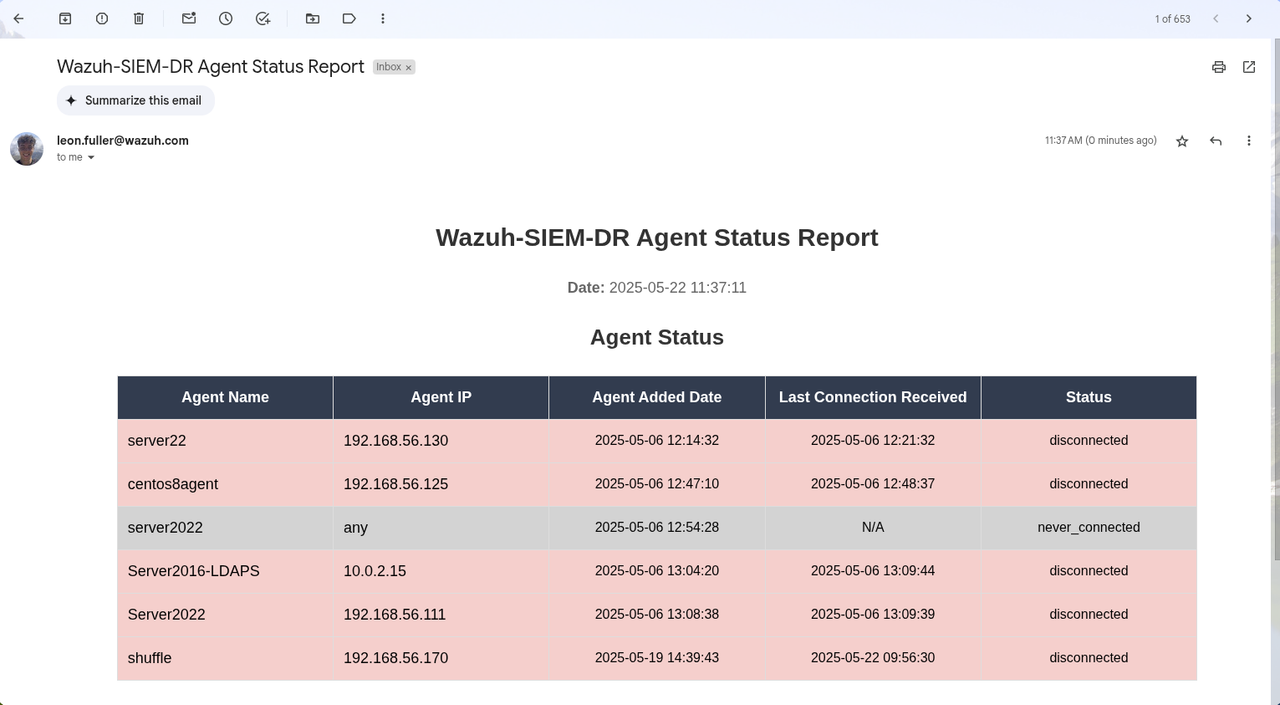
\includegraphics[width=1.0\textwidth]{figures/wazuh_agent_report_example.png}
  \caption{Ejemplo de reporte diario de estado de agentes (formato HTML renderizado).}
  \label{fig:agent_report}
\end{figure}

Este enfoque basado en Bash garantiza alta difusión y compatibilidad en múltiples sistemas Linux, evitando la complejidad y las dependencias de un entorno Python, y facilita la obtención de estadísticas diarias sin intervención manual.  
    \chapter{Valoración Personal}

\section{Asignaturas Relacionadas}
Para la ejecución de las tareas anteriores, resultaron fundamentales los conocimientos de las siguientes asignaturas del plan de estudios:
\begin{itemize}
  \item \textbf{Sistemas Operativos}: Configuración avanzada de Linux y Windows, administración de servicios, scripting en Bash y PowerShell.  
  \item \textbf{Ingeniería de Servidores}: Fundamentos de criptografía, detección de intrusiones, gestión de incidentes y aplicación de estándares de seguridad (PCI DSS, HIPAA).  
  \item \textbf{Fundamentos de Redes}: Protocolos TCP/IP, configuración de firewalls, conceptos de IDS/IPS y análisis de tráfico con Wireshark/Suricata.  
  \item \textbf{Fundamentos de Bases de Datos}: Ingesta y consulta de grandes volúmenes de datos (alertas) en Elasticsearch/OpenSearch, optimización de índices y consultas.  
  \item \textbf{Ingeniería de Software}: Diseño de arquitecturas distribuidas, uso de herramientas de control de versiones (Git) y metodologías ágiles en proyectos de DevOps.  
\end{itemize}

\section{Valoración de la Experiencia}
Durante el periodo de prácticas en Wazuh, pude adquirir competencias prácticas en despliegue y administración de soluciones SIEM/XDR, así como en el desarrollo e implementación de reglas de detección basadas en estándares de ciberseguridad. La exposición continua a entornos empresariales reales y la colaboración con profesionales de distintas áreas fortalecieron mi capacidad para trabajar bajo presión y resolver problemas complejos de manera eficiente.

He de destacar que entré en un equipo donde no había un jefe, es decir, en cada equipo de zona horaria hay un jefe del mismo, que se encarga de organizar, vigilar y ayudar a sus subordinados. Yo tuve que reportar directamente al jefe de todo el equipo de Operaciones. Esto hizo que mi recorrido sea más difícil, no obstante, tuve la ayuda necesaria y pude completar todos los obstáculos y retos que me encontré por delante.
    \chapter{Conclusiones}
Durante estos tres meses de prácticas en Wazuh he tenido la oportunidad de colaborar con equipos multidisciplinares y entender en profundidad la organización y el funcionamiento de una empresa tecnológica de gran envergadura. Este periodo me ha permitido adquirir una visión amplia tanto del ámbito corporativo como del técnico, y experimentar de primera mano cómo se gestionan proyectos complejos en un entorno real. He aprendido a trabajar con herramientas y tecnologías punteras en ciberseguridad, tales como Kubernetes (EKS y entornos autogestionados), Terraform y Ansible para la provisión y configuración de infraestructura en AWS y OpenSearch/Elasticsearch para la indexación y análisis de logs. Asimismo, reforcé mis conocimientos sobre el despliegue de Wazuh Manager y Wazuh Agent en arquitecturas de alta disponibilidad, manejo de volúmenes persistentes y certificados TLS en entornos distribuidos. Gracias al soporte continuo de la comunidad open source de Wazuh (Reddit, Discord, Slack, GitHub), pude consultar y resolver rápidamente dudas, lo que facilitó enormemente la integración de buenas prácticas y soluciones ya contrastadas.

Por otro lado, he mejorado significativamente mi comprensión de los conceptos de redes y protocolos: aprendí a diagnosticar problemas con \texttt{tcpdump}, interpretar el intercambio de paquetes TCP (SYN, SYN–ACK, RST), configurar reglas de \texttt{iptables} para permitir tráfico SMTP y depurar conexiones SMTP/TLS con Postfix. Asimismo, profundicé en el uso de APIs REST de Wazuh, autenticación con tokens JWT, scripting avanzado en Bash (manipulación de JSON con \texttt{jq}, construcción dinámica de HTML/CSS, manejo de fechas y registros), y configuración de \texttt{cron} para automatizar tareas diarias. Esta experiencia global me ha dotado de un conjunto de competencias técnicas sólidas en administración de sistemas Linux, orquestación de contenedores, herramientas de automatización, gestión de seguridad en la nube y metodologías de diagnóstico y monitorización, que sin duda fortalecerán mi perfil profesional y me preparan para afrontar nuevos retos en el ámbito de la ciberseguridad y la ingeniería de infraestructura.
  \backmatter
    \bibliographystyle{apalike}
    \bibliography{bibliography}
\end{document}
